\begin{table*}[h]
	\centering
	\caption{Benchmarks and descriptions}
	\label{table:benchmarks}
	\begin{tabular}{|p{0.1\textwidth}|p{0.06\textwidth}|p{0.16\textwidth}|p{0.4\textwidth}|p{0.08\textwidth}|p{0.11\textwidth}|}
		\toprule
		Name & \ac{ANN} Type                 & Real-time Classification                             & Description                                                   & \#\acp{ANN} & \#Neurons \\ \midrule
		AI-BRO & \ac{MLP}           & Hard real-time                            & The steering controller described in Section~\ref{sec:motivating-example}.                 & 3      & (11, 11, 13)      \\
		ESS & \ac{MLP}   & Hard real-time & Controls an EV charging station with a storage battery. & 3     & (74, 23, 18)      \\
		XOR & \ac{MLP} & Hard real-time                            & Performs Exclusive-Or of two boolean inputs.                 & 1      & 6      \\
		ADDER & \ac{MLP}          & Hard real-time              & Adds two 31-bit numbers together.              & 1      & 5           \\ 
		HELLO & \ac{RNN}     & Hard real-time              & \ac{RNN} trained to remember the letters of `hello'. & 1      & 14      \\
		RABBIT & \ac{MLP}     & Soft real-time              & Turn based, zero-sum game played between two teams of \acp{ANN} & 3      & (50, 60, 60)      \\
		SENSOR & \ac{CNN}     & Soft real-time              & Section~\ref{sec:motivating-example} front sensor implementation for object detection using images. & 1      & 1000+      \\
		\bottomrule
	\end{tabular}
\end{table*}

\section{Case studies and evaluation}
\label{sec:results}
%\pr{I have defined the concept of reaction time and response time. We
%  should have both these in all real-time benchmarks and accordingly
%  evaluate the results.}

We have developed a set of benchmark applications, written in Esterel,
to evaluate the efficacy of the developed approach. These benchmarks are presented in Table~\ref{table:benchmarks}, and are also
publicly available at \textit{https://github.com/PRETgroup/sann}. All benchmarks in this paper were developed in Esterel, C, and where appropriate, Python. 
Hard-real time benchmarks were analysed using the timing analysis tool
Platin~\cite{compiler:platin:kps15}, 
and executed on a Patmos soft-core processor~\cite{patmos:ppes2011} 
on an Altera DE2-115 FPGA running at 50MHz. 
All neural networks were trained offline (i.e. pre-trained).

The benchmarks include an Energy
Storage System (\texttt{ESS}) inspired by~\cite{chaudhari2017hybrid},
the \texttt{AI-BRO} example from Section~\ref{sec:motivating-example}, the \texttt{XOR} network from Section~\ref{sec:esterel-mapping}, and an \texttt{ADDER} developed for
pedagogy. These examples all use \ac{MLP}-based
\acp{SANN}. We have also developed an example involving a \ac{RNN}
called \texttt{HELLO}. 
These first benchmarks are all statically analysed to
compute their \ac{WCRT} and hence could be used in hard real-time
applications. The \texttt{ESS} example is the most complex of these
benchmarks, as it illustrates the concept of meta neural networks
(Section~\ref{sec:concurrent-sann}) involving three neural networks
with 74, 23, 18 neurons respectively.

As this is the first work on synchronous neural networks, we had to
develop time analysable implementations from scratch. Unfortunately, we were unable
to complete the implementation of more complex \acp{ANN} such that they met the requirements of the Platin tool. 
However, we did develop two additional interesting soft-real time examples to illustrate the power of the proposed methodology. The
first example is a computer game called \texttt{RABBIT}, which was
also implemented using Pthreads in Python.
This program demonstrates the
benefits of the synchronous approach. 
Lastly, we developed a \ac{CNN} application called \texttt{SENSOR}, by reusing
libraries from Darknet~\cite{redmon2015real}. This example involved more than 1000 neurons, and we
were able to implement both the ``black box'' and the ``layer by layer'' approaches.

\ignore{
	and have been developed keeping the 
	Two types of \acp{CPS} were considered for this paper: those that are hard-real time, and need their \ac{WCRT} derived, and those that have soft real-time deadlines which can just be measured instead.
	The full suite of these benchmarks are presented in Table~\ref{table:benchmarks}, and are also
	publicly available at \todo{link}. 
	In this section, we discuss these results in more detail.}

%\subsection{Methodology}



%\subsection{An \acf{ESS} System}
\paragraph{An Energy Storage System \texttt{ESS}}
\label{sec:ess}
\acf{ESS} are used to lower the costs of
charging an electric vehicle (EV)~\cite{chaudhari2017hybrid}. %\pr{Please cite the TII journal version.}
Simply put, an \ac{ESS} serves as an intermediary between the electrical grid and a large electrical load i.e. an EV.
Usually, it is made up of a connection to the grid, a connection to
the load, one or more electrical storage devices (such as batteries), and a controller to manage the system, as 
depicted in Figure~\ref{fig:ess-components}.

\begin{figure}[b]
	\vspace{-3mm}
	\centering
	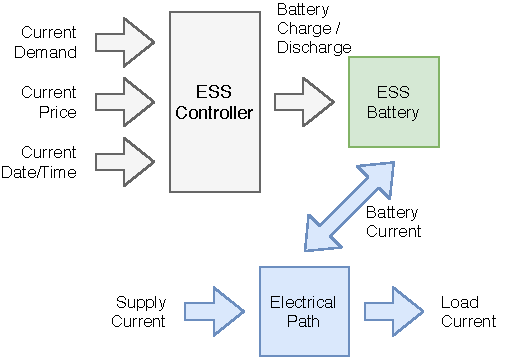
\includegraphics[scale=0.68]{Content/fig/ess_components}
	\caption{Example \ac{ESS} Components\label{fig:ess-components}}
\end{figure}

\acp{ESS} work by shifting the burden of their electrical load to the
electrical grid during periods of low demand, i.e. when the price is the cheapest.
Then, as the load on the grid increases along with consequent increase
in price, the \ac{ESS} starts to supply its load from its battery instead. 
This results in a lower average cost for providing the load current. 
This system must be functionally correct while also meeting timing
deadlines i.e.
the system must respond to safety situations within a time bound. 

Our \texttt{ESS} has an associated
over-current detector.  When this triggers, the system must evade this
unsafe situation within 30 milli-seconds to activate a circuit
breaker, which must take effect within this deadline. 
However, the response time of the overall \texttt{ESS} controller is much less strict, as it has a soft-real time \textit{quality of service} deadline of one second.
This is primarily because the demand input of the \texttt{ESS} does not need to be sampled faster than every second for suitable behaviour.
In addition, the price of electricity changes only once every 10 minutes.
%  \pr{You may also
%  add the response time requirement upfront, which is from input to
%  the corresponding output of a given \ac{SANN}.}

\ignore{Deciding when to charge and discharge an \ac{ESS} battery is non-trivial. 
	There are many factors to consider, including the current \ac{SoC} of the battery, historical data on pricing and load demand current.
	A variety of approaches have been used, including statistical modelling in \cite{TOUESS}.
	%In addition, a system that is in charge of a battery must include
	%safety features, i.e. an electrical over-current detector, to ensure
	%that the users of the \ac{ESS} remain safe at all times: In the event
	%of an over-current, the industry standard requires that this unsafe
	%situation should be evaded within 30ms. 
}

We propose a meta neural network, involving three 3-layer \ac{MLP} \acp{SANN}, to decide when to charge and discharge the battery in our \texttt{ESS}.
These networks operate synchronously with a over-current detector
that preempts the system by activating a circuit breaker.
The architecture of this meta neural network is presented in Figure~\ref{fig:ess-sanns}. 
%In this case, 
%Using the ``layer by layer'' approach, we can guarantee a low \ac{WCRT} to ensure safety in the face of an electrical over-current, 
%as the \textit{Safety Cutoff} heuristic will be evaluated in each synchronous tick.

\begin{figure}
	\centering
	\scalebox{0.7}{\begin{tikzpicture}[->,>=stealth',shorten >=1pt,auto,
node distance=3cm,
semithick,scale=0.8, transform shape,scale=0.6, font=\huge]

\tikzstyle{every state}=[rectangle, text width=3cm, minimum height=1cm, text centered, 
fill=blue!20,draw=none,text=black, draw,line width=0.3mm, font=\LARGE]

%start state
\node[state,fill=none]
(cdemand)
{Demand}; 

\node[state,fill=none]
(ctime) [below of=cdemand]
{Date/Time};

\node[state,fill=none]
(cprice) [below of=ctime]
{Price}; 

\node[state,fill=none]
(csoc) [below of=cprice]
{ESS SoC}; 

\node[state,fill=none]
(ccur) [below of=csoc]
{Outflow Current}; 

\node[state]
(prdemand) [right of=cdemand, xshift=2cm, yshift=-1.5cm]
{Predict Demand}; 

\node[state]
(prprice) [below of=prdemand]
{Predict Price}; 

\node[state]
(ess) [right of=prprice, xshift=2cm, yshift=-1.5cm]
{Manage ESS};

\node[state,fill=red!20]
(scut) [right of=ccur, xshift=4.5cm]
{Safety Cutoff}; 

\node[state,draw=none, fill=none]
(parallel) [above of=scut]
{\texttt{||}}; 

\node[state,fill=none]
(essoutp) [right of=ess, xshift=2cm]
{Battery Command};

\node[state,fill=none]
(breaker) [right of=scut, xshift=4.5cm]
{Breaker Command};

\path[->] (cdemand) edge (prdemand);
\path[->] (ctime) edge (prdemand);
\path[->] (ctime) edge (prprice);
\path[->] (cprice) edge (prprice);
\path[->] (cprice) edge (ess);
\path[->] (prdemand) edge (ess);
\path[->] (prprice) edge (ess);
\path[->] (csoc) edge (ess);
\path[->] (ess) edge (essoutp);
\path[->] (ccur) edge (scut);
\path[->] (scut) edge (breaker);

\draw[->] (cdemand.east)  
	|- ($(cdemand.east) + (5cm, 0)$) 
	-\ (ess.north);
	
\draw[-,dashed] ($(prdemand.north) + (-2.5cm, 0.5cm)$) 
-| ($(ess.east) + (0.5cm, 0)$) 
|- ($(ess.south) + (0, -0.5cm)$)
-| ($(prdemand.north) + (-2.5cm, 0.5cm)$);

\draw[-,dashed] ($(scut.north) + (-5cm, 0.5cm)$) 
-| ($(scut.east) + (3cm, 0)$) 
|- ($(scut.south) + (0, -0.5cm)$)
-| ($(scut.north) + (-5cm, 0.5cm)$);

\end{tikzpicture}
}
	\caption{ESS \ac{SANN} / Safety Cutoff arrangement}
	\label{fig:ess-sanns}
\end{figure}

Training this system complex, as it is not
feasible to provide all possible correct commands for every possible
input. Hence, back-propagation could not be used.
Instead, Q-learning~\cite{qlearning2010}, a type of reinforcement learning, was used for training the network.
\ignore{ Reinforcement learning trains an \ac{ANN} without knowledge of the
	correct output. 
	
	It trains based on the reinforcement of the reward of any given action $A$, with regard to the current state $S$. 
	An action that is \emph{good} will be given a high reward, and the \ac{SANN} will get its weights updated in an attempt to preserve the behaviour.
	A \emph{bad} action, however, will result in the  weights being modified so that it will have a reduced chance of choosing that action in that state again. 
	Using this system, Q-learning attempts to train an \ac{SANN} to follow the path of highest reward.}


%In our case, demand and price were modelled as sine functions, and the networks were trained with the goal of reducing the overall ``real-world'' cost \pr{I don't understand what you mean here?}
%of outputting energy from the \ac{ESS} system. 
%The \ac{ESS} was rewarded for buying energy when it was cheap, and supplying it when it was expensive.

In order to validate this design, we performed \ac{WCRT} analysis of
both the mono-periodic and multi-periodic implementations. 
%\pr{What
%  was the length of the multi period? For all these benchmarks, we
%  have to state the length of the period and the how many cycles are
%  needed. In particular, we have to state from input to output how
%  long it takes for all approaches.}
These results are presented in Table~\ref{tbl:res-ess}.

\begin{table}[H]
	\centering
	\caption{\ac{WCRT} results for \texttt{ESS}}
	\label{tbl:res-ess}
	\begin{tabular}{|l|l|l|}
		\hline
		Approach         & WCRT (ms) & Response Time (ms)\\ \hline
		Black-box        & 14   & 14 \\ 
		Layer by layer   & 9.8  & 58.8 \\ \hline
	\end{tabular}
\end{table}

As can be seen, the \ac{WCRT} for the mono-periodic ``black-box''
approach is $14ms$, 
making the total worst-case cut-off time $28ms$ (one cycle to capture value, one cycle to emit command).
This only gives $2ms$ for the hardware to respond to a digital signal
to cut the circuit, which may not be sufficient.

Considering this, we developed  a multi-cyclic ``layer by layer''
approach, that results in a \ac{WCRT} of $9.8ms$, 
giving a total worst-case cut-off time time of $<20ms$. 
This gives sufficient time for the physical hardware to respond and break the circuit.
In addition, although changing the implementation to multi-cyclic does increase the \ac{ANN} response time by $54.8$ms, it does not
come close to the deadline of the \ac{ESS} battery command, which has a one second soft-real time deadline.

\paragraph{\texttt{AI-BRO}}
%\subsection{AI-BRO} 
Introduced in Section~\ref{sec:motivating-example}, and as depicted in Figure~\ref{fig:av}, \texttt{AI-BRO} uses three different \acp{SANN} working together to guide an automatic vehicle. 
For this case study, the \acp{SANN} were simple \acp{MLP}.
Each was trained using back-propagation with a gradient descent approach~\cite{yegnanarayana1994artificial}, as the correct outputs for each of the inputs could be exactly specified.
For instance, \texttt{AI-BRO}, a front sensor reading of $(010)_2$ implies an obstacle directly in front of the vehicle.
Therefore, the vehicle must either turn left, turn right, or stop.
%\changed{\sout{The front \ac{SANN} is responsible for passing this information to the driver \ac{SANN}.}}
Consequently, it should output $(101)_2$.
%The first network takes input from the frontal sensors. These consist of 3 boolean values.
%Then, it outputs an initial suggestion for the car to travel, as an enumerated value across 3 bits for 6 different actions \textit{\{stop, stop/turn left, stop/turn right, turn left, turn right, continue straight\}}.

%Like the first network, the second \ac{SANN} also processes sensor data. 
%This time, the inputs are boolean values coming from the side sensors.
%A single boolean output for each side indicates whether or not a given direction is obstructed.

%The third and final \ac{SANN} takes in the outputs from the two sensor-processing networks. 
%Using the information they provide, it makes the actual decision for the car to follow.


Once created, \ac{WCRT} values were able to be derived for both mono-cyclic and multi-cyclic implementations, and are provided in Table~\ref{tbl:res-aibro}.

\begin{table}[H]
	\centering
	\caption{\ac{WCRT} results for \texttt{AI-BRO}}
	\label{tbl:res-aibro}
	\begin{tabular}{|l|l|l|}
		\hline
		Approach         & WCRT (ms) & Response Time (ms)\\ \hline
		Black-box        & 2.8  & 2.8  \\ 
		Layer by layer   & 1.9  & 11.4 \\ 
		Neuron by neuron & 1.8  & 10.8 \\ \hline
	\end{tabular}
\end{table}


\paragraph{\texttt{XOR} / \texttt{ADDER}}
%\subsection{XOR / ADDER}
\label{sec:xor-and-adder}

In addition to the exclusive-or \ac{MLP} \texttt{XOR} used as an example in Sections
\ref{sec:esterel-mapping} and \ref{sec:concurrent-sann},
an \ac{MLP} \texttt{ADDER} was also created that could add two 31-bit numbers together. 
These two networks were both straightforward to train and analyse 
due to their simple 3-layer designs, and their \acp{WCRT} are presented in Table~\ref{tbl:res-xor-adder}.

\begin{table}[H]
	\centering
	\caption{\ac{WCRT} results for \texttt{XOR} and \texttt{ADDER}}
	\label{tbl:res-xor-adder}
	\begin{tabular}{|l|l|l|}
		\hline
		Approach         & WCRT (ms) & Response Time (ms)\\ \hline
		\multicolumn{3}{|l|}{\texttt{XOR}}  \\ \hline
		Black-box        & 0.82 & 0.82   \\ 
		Layer by layer   & 0.57 & 1.71  \\ 
		Neuron by neuron & 0.6  & 1.8 \\  \hline
		\multicolumn{3}{|l|}{\texttt{ADDER}}  \\ \hline
		Black-box        & 0.49 & 0.49   \\ 
		Layer by layer   & 0.39 & 1.17  \\ 
		Neuron by neuron & 0.33 & 0.99 \\  \hline
	\end{tabular}
\end{table}

\paragraph{\texttt{HELLO}}
%\subsection{HELLO}

The \texttt{HELLO} system is a 3-layer \ac{RNN} which was trained to learn the pattern of the word ``hello''. 
We implemented this system to demonstrate that the synchronous
approach works with any type of \acp{ANN}, not just \acp{MLP}.
The results of this system are presented in Table~\ref{tbl:res-hello}.

\begin{table}[H]
	\centering
	\caption{\ac{WCRT} results for \texttt{HELLO}}
	\label{tbl:res-hello}
	\begin{tabular}{|l|l|l|}
		\hline
		Approach         & WCRT (ms) & Response Time (ms)\\ \hline
		Black-box        & 2.22  & 2.22  \\ 
		Layer by layer   & 1.33  & 3.99  \\ \hline
	\end{tabular}
\end{table}


\paragraph{\texttt{RABBIT} and \texttt{SENSOR}}
%\subsection{RABBIT}

%\pr{Is this a well known game? Citation needed}.


\ignore{The game is played in turns between two teams: wolves and a rabbit who
	are moving in a map. The wolves play on the same turn, working
	together to catch the rabbit. 
	The rabbit plays alone and attempts to escape the map. The wolves play on the same turn, working together to
	catch the rabbit. The rabbit scores if it leaves the map before time
	runs out. The wolves, on the other hand, win if they catch the
	rabbit before time runs out. The game runs in a loop. At the
	start of every round, all animals decide \textit{at the same time}
	where they will move too. 
	The system then updates and computes the score accordingly. Unless
	there was a winner, or time ran out, the 
	iterations continue.}

The \texttt{RABBIT} game was designed to highlight the benefits of synchronous
programming while designing meta neural networks. 
The game is played in turns between two teams, wolves and a rabbit, who
are moving in a map.
Each animal in the game has its own functional \ac{ANN}, which operate synchronously, respecting causality and avoiding deadlocks. 
The same system was also implemented in Python (using
Pthreads), without the use of any synchronization primitives, and we found
that the %\changed{\sout{
%We used
%these examples to evaluate the correlation coefficient between the
%Python and the Esterel implementation and found that the }
outputs of the two versions were
strongly correlated. %}

\ignore{The \acp{ANN} were run concurrently on separate Pthreads and the system updated after each \ac{ANN} thread finished running. 
	Although uncommon, it was noted that the Pthread implementation was
	susceptible to producing scores that should have been impossible
	for the system to attain. For example, the rabbits and wolves scoring on the same turn; this should not be possible, as either the wolves win or the rabbit, but not both. This was due to the disregard for causality in the
	running of Python's threads. \pr{I am unclear what you are claiming
		here. What is an impossible score and why? Are you referring to
		typical race conditions?}
	
	%Unfortunately this system is not currently time analysable using Platin. The system was originally implemented without regard to the timing analysis guidelines of \acp{SANN} as listed in Section~\ref{sec:wcrt}. As a result, this system contains some code that prevents WCET analysis at this time.
	
	Due to the large number of neurons in the \acp{ANN} of this system, one of the wolf \ac{ANN} was used to calculate the correlation coefficient between an Esterel implementation of an \ac{ANN}, i.e. \ac{SANN}, and an asynchronous \ac{ANN} using the exact same weights.
	
	The results of these calculations are presented in Table~\ref{tbl:res-game}.
	\begin{table}[H]
		\centering
		\caption{Correlation coefficient results for \texttt{RABBIT}}
		\label{tbl:res-game}
		\begin{tabular}{|l|l|}
			\hline
			Coefficient & Value \\
			\hline
			Pearson & 0.999999802345 \\
			\hline
		\end{tabular}
	\end{table}
	
	\paragraph{SENSOR}
	%\subsection{SENSOR}
}


\acp{DNN} have many industrial applications compared to any other type
of \ac{ANN}. This is largely due to their ability to train to
extremely large amounts of data. We implemented a \texttt{SENSOR}
application using a \ac{DNN}. An open source library called Darknet~\cite{redmon2015real} was used
to implement this \ac{CNN}. Darknet provides a platform for training
of many types of \acp{ANN} in C, including \acp{CNN}. 
%\changed{\sout{Using an already trained \ac{CNN} that can perform object recognition
%on input images, an Esterel system was created to run this \ac{CNN}, using the
%mentioned blackbox approach and the layer--by--layer approach.}
Using this system, an Esterel application was developed to recognize images using the black-box and the layer by layer approaches.%}

\begin{table}[H]
	\centering
	\caption{Combined \ac{WCRT} results for \texttt{ESS}, \texttt{AI-BRO}, \texttt{XOR}, \texttt{ADDER} and \texttt{HELLO}}
	\label{tbl:res-sann}
	\begin{tabular}{|l|l|l|l|}
		\hline
		Approach         & WCRT (ms) & Response Time (ms) & Size (neurons) \\ \hline
		\multicolumn{4}{|l|}{\texttt{ESS}} \\ \hline
		Black-box        & 14  & 14 & 125 \\ 
		Layer by layer   & 9.8  & 58.8 & 125 \\
		MNN2C			 & 4.41 & 4.41 & 125 \\ \hline
		\multicolumn{4}{|l|}{\texttt{AI-BRO}}  \\ \hline
		Black-box        & 2.8  & 2.8 & 35 \\ 
		Layer by layer   & 1.9  & 11.4 & 35 \\ 
		Neuron by neuron & 1.8  & 10.8 & 35 \\ 
		MNN2C			 & 2.29 & 2.29 & 35 \\ \hline
		\multicolumn{4}{|l|}{\texttt{XOR}}  \\ \hline
		Black-box        & 0.82 & 0.82 & 6  \\ 
		Layer by layer   & 0.57 & 1.71 & 6 \\ 
		Neuron by neuron & 0.6  & 1.8 & 6 \\ 
		MNN2C			 & 0.53 & 0.53 & 6 \\ \hline
		\multicolumn{4}{|l|}{\texttt{ADDER}}  \\ \hline
		Black-box        & 0.49 & 0.49 & 5  \\ 
		Layer by layer   & 0.39 & 1.17 & 5 \\ 
		Neuron by neuron & 0.33 & 0.99 & 5 \\ 
		MNN2C			 & 0.37 & 0.37 & 5 \\ \hline
		\multicolumn{4}{|l|}{\texttt{HELLO}}  \\ \hline
		Black-box        & 2.22  & 2.22 & 14 \\ 
		Layer by layer   & 1.33  & 3.99 & 14 \\ \hline
	\end{tabular}
\end{table}

\ignore{
	\pr{How
		many layers? Can we give some measurement-based timing analysis
		results for the game and the CNN?}
	The system ran through 16 layers, taking approximately 500ms for all 16 layers to run. This time was taken by measurement and is not a WCET value. Although no WCET analysis was possible, due to the open source library not following any of the timing analysis guidelines listed in Section~\ref{sec:wcrt}, the system was able to run in Esterel. This shows that the synchronous implementation of \acp{DNN} using C and Esterel is not only possible, but that the whole range of \acp{ANN} can be implemented synchronously using the Esterel programming language.
}













